\section*{Part 1}
Since we are dealing with a robotic arm, the angles $\alpha$ and $2\pi+\alpha$ are equivalent in the final position, therefore in this solution we restrict to $\theta_i \in [-\pi,\pi) , i\in \{1,2,3\}$. 

\begin{comment}
\begin{figure}
    \centering
    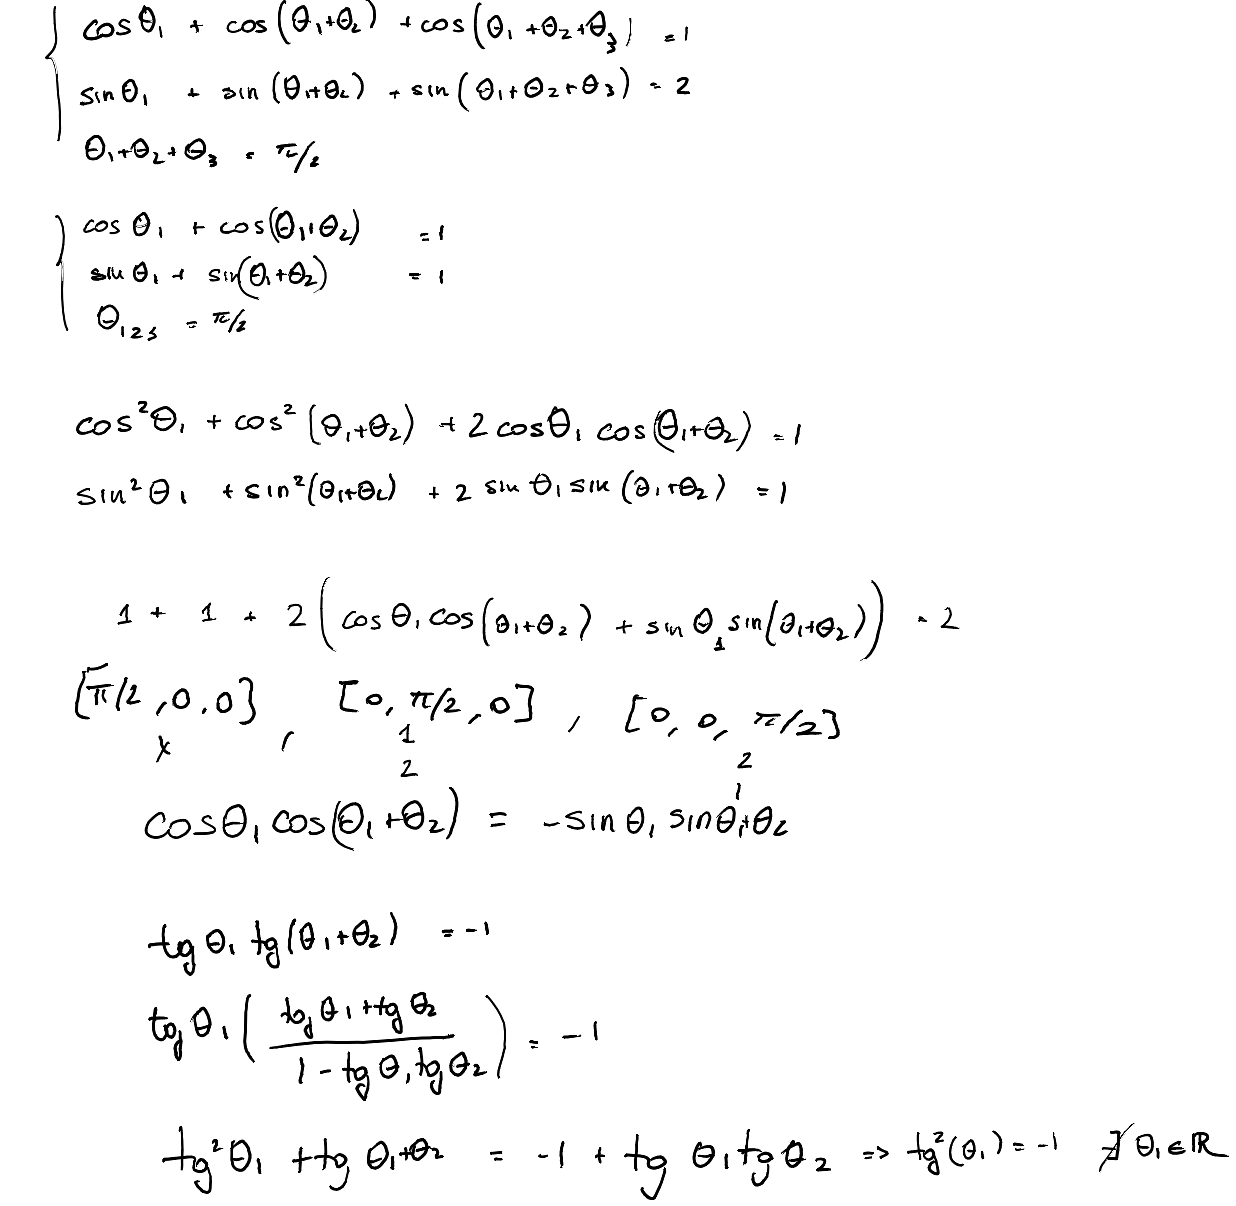
\includegraphics[width=0.5\linewidth]{Base.png}
\end{figure}
\end{comment}


To find the angles $\vec\theta=[\theta_1\, \theta_2 \, \theta_3]^\top$, we need to solve the following system
$$\begin{cases}
    \cos(\theta_1) + \cos(\theta_1+\theta_2) + \cos(\theta_1+\theta_2+\theta_3) = 1 \\ 
    \sin(\theta_1) + \sin(\theta_1+\theta_2) + \sin(\theta_1+\theta_2+\theta_3) = 2\\ 
    \theta_1+\theta_2+\theta_3 = \dfrac{\pi}{2}
\end{cases}$$
Therefore from the last equation, we can simplify the model to 
$$\begin{cases}
    \cos(\theta_1) + \cos(\theta_1+\theta_2)  = 1 \\ 
    \sin(\theta_1) + \sin(\theta_1+\theta_2) +1 = 2\\ 
    \theta_1+\theta_2+\theta_3 = \dfrac{\pi}{2}
\end{cases}$$
By squaring both sides and summing the first two equations, we get 
$$ 1+1+2\bigg(\cos(\theta_1)\cos(\theta_1+\theta_2) + \sin(\theta_1)\sin(\theta_1+\theta_2) \bigg) =2$$
Which implies that 
\begin{equation*}
   \cos(\theta_1)\cos(\theta_1+\theta_2) = - \sin(\theta_1)\sin(\theta_1+\theta_2) \tag{$\star$}
\end{equation*}
This is equivalent to $\tan(\theta_1)\tan(\theta_1+\theta_2) = -1$ only if the two cosines are not equal to zero, therefore there are three (+ 1) subcases starting from $\star$: the first one is if neither of them is different form zero, if $\cos(\theta_1) = 0$ and the other two arise when $\cos(\theta_1+\theta_2) = 0$. 
\begin{comment}
\begin{figure}
    \centering
    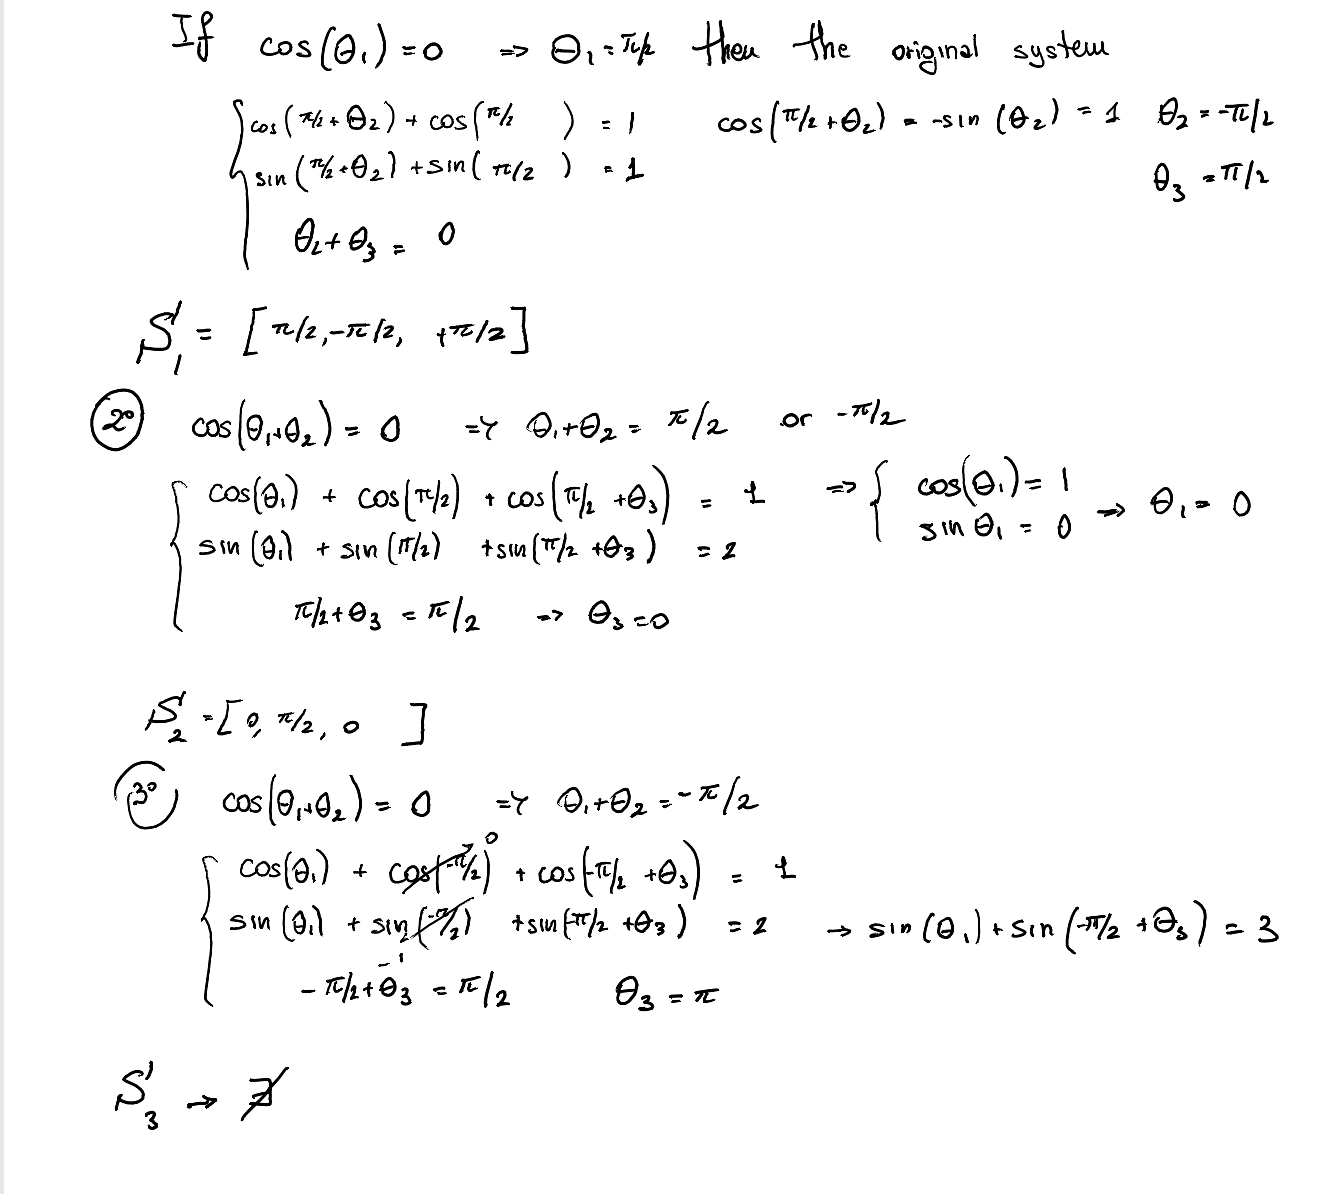
\includegraphics[width=0.5\linewidth]{Casistiche.png}
\end{figure}
\end{comment}
\newpage
\begin{tcolorbox}[title={Case 1: $\cos(\theta_1)=0$}, colback=blue!5, colframe=blue!40!black, breakable]
$\theta_1 = \tfrac{\pi}{2}$ and $\theta_2+\theta_3=0$. Substituting:
\[
\begin{cases}
    \cos\!\left(\tfrac{\pi}{2}+\theta_2\right) = 1 \;\Longrightarrow\; -\sin\theta_2=1\\[4pt]
    \sin\!\left(\tfrac{\pi}{2}+\theta_2\right) = 1 \;\Longrightarrow\; \cos\theta_2=0
\end{cases}
\quad\Longrightarrow\quad \theta_2 = -\frac{\pi}{2},\quad \theta_3=\frac{\pi}{2}
\]
\tcblower
\centering $\displaystyle S_1 = \left[\frac{\pi}{2},\,-\frac{\pi}{2},\,\frac{\pi}{2}\right]^\top$
\end{tcolorbox}
 
\medskip
 
\begin{tcolorbox}[title={Case 2: $\cos(\theta_1+\theta_2)=0$ with $\theta_1+\theta_2=+\pi/2$}, colback=green!5, colframe=green!40!black, breakable]
$\cos(\pi/2)=0$, $\sin(\pi/2)=1$, and $\theta_3=0$. The system gives:
\[
\begin{cases}
    \cos\theta_1 + 0 = 1\\[4pt]
    \sin\theta_1 + 1 = 1
\end{cases}
\quad\Longrightarrow\quad \theta_1=0,\quad \theta_2=\frac{\pi}{2},\quad \theta_3=0
\]
\tcblower
\centering $\displaystyle S_2 = \left[0,\,\frac{\pi}{2},\,0\right]^\top$
\end{tcolorbox}
\begin{tcolorbox}[title={Case 3: $\cos(\theta_1+\theta_2)=0$ with $\theta_1+\theta_2=-\pi/2$}, colback=red!5, colframe=red!40!black, breakable]
$\cos(-\pi/2)=0$, $\sin(-\pi/2)=-1$, and $\theta_3=\pi$. The second equation becomes:
\[
\sin\theta_1 + (-1) + \sin\!\left(\frac{\pi}{2}\right) = 2 \quad\Longrightarrow\quad \sin\theta_1 = 2 \quad\Longrightarrow\quad \nexists\,\theta_1\in\mathbb{R}
\]
\tcblower
\centering No solution.
\end{tcolorbox}

\begin{tcolorbox}[title={Case 4: everything goes well} , colback=orange!5, colframe=orange!70!black, breakable]
Using $\tan(a+b) = \frac{\tan a + \tan b}{1 - \tan a \tan b}$: 
$$\tan(\theta_1)\frac{\tan \theta_1 + \tan \theta_2}{1 - \tan \theta_1 \tan \theta_2} = -1$$
Which means solving the quadratic equation $$\tan^2\theta_1 + \cancel{\tan(\theta_1+\theta_2)}=-1 +\cancel{\tan(\theta_1+\theta_2)} \implies \nexists \, \theta_1\in\mathbb{R}$$. 
\tcblower
\centering No solution.
\end{tcolorbox}

Hence, there are only two solutions:  \\

\begin{figure}[H]
\centering
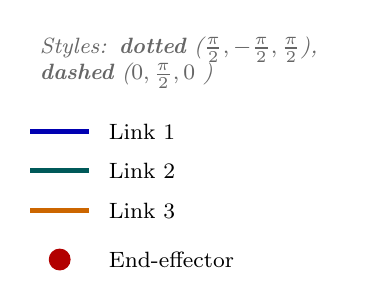
\begin{tikzpicture}[scale=2.5]
  % ── Soluzione 1: theta = [pi/2, -pi/2, pi/2]
  %    cumulative angles: phi1=90, phi2=0, phi3=90
  \begin{scope}[xshift=0cm]
    \drawarm{90}{0}{90}{}{my dotted}
    \drawarm{0}{90}{90}{}{dashed}
  \end{scope}
  % shared legend

  \begin{scope}[xshift=2.2cm, yshift=1.8cm] % Spostata più a destra per dare respiro

    \node[right, font=\footnotesize\itshape, text width=4cm] at (0, 0.15) 
      {\textcolor{black!60}{Styles: \textbf{dotted} ($\frac\pi2, -\frac\pi2, \frac\pi2$), \textbf{dashed} ($0,\frac\pi2,0$ )}};
    
    \foreach \col/\lbl/\y in {
        blue!70!black/Link 1/ -0.2,
        teal!70!black/Link 2/ -0.4,
        orange!80!black/Link 3/ -0.6}{
      \draw[\col, line width=1.8pt] (0,\y) -- (0.3,\y);
      \node[right, font=\footnotesize] at (0.35,\y) {\lbl};
    }
    
    \filldraw[red!70!black] (0.15, -0.85) circle (1.5pt);
    \node[right, font=\footnotesize] at (0.35, -0.85) {End-effector};
  \end{scope}
\end{tikzpicture}
\caption{This picture displays the two solutions (they both reach the point $(1,1)$ but follow two different paths (dotted and dashed), from there they reach point $(1,2)$ (dash dotted) }
\end{figure}

 